\chapter{课外实验活动}
\setcounter{section}{0}
\section{观察扩散现象}

在容器里装一半水,然后用长颈漏斗小心地把硫酸铜溶液倒进容器的底部,硫酸铜溶液比水的密度大,沉在容器下部,可以看到无色的水和蓝色的硫酸铜溶液的界面非常清楚.由于扩散,经过几天以后,界面上方的水变蓝,界面下方的溶液的颜色变浅,界面变得模糊了,经过更长的时间,全部溶液将变成均匀一致的颜色.把装有水和硫酸铜溶液的容器放在不容易碰到的地方,每隔一天,按时观察现象,看看要多长时间全部液体才变成均匀一致的颜色.

\section{自制冰淇淋}
冰和盐的混合物的熔点可以降到零下二十多摄氏度,因
此可以用冰盐混合物进行冷却,现在我们用冰盐混合物致冷来自制冰淇淋.

制冰淇淋需要的原料有牛奶、鸡蛋、玉米粉、糖以及其他香料,把配好的原料\footnote{原料的配法:把生鸡蛋打开放在碗里,加入少许玉米粉搅匀.然后慢慢冲入煮沸的加糖牛奶并且要边冲边搅.最后,放入香料,再用锅稍稍熬一会儿,冷却后即成.}放在小铝锅里.找一个大容器(如一只大锅),里面装冰盐混合物(大致是三份冰,一份盐的比例)或雪盐混合物,把小铝锅放在冰盘混合物中,只有锅盖露在外面.过一些时间打开锅盖,看看是否快要冻结.当快要冻结时要
搅拌,否则结成的冰粒很粗,不好吃;也不要冻结得太厉害,因为冻得太硬,也不好吃.

\section{人造云雾}
用冰盘混合物致冷可以人工造成云雾.找一个小铁罐(如一个罐头盒子),放在冰盐混合物或雪盐混合物中,小铁罐里的空气很快就冷却,对着小铁罐吹口气,水蒸气就被带进铁罐里,由于里面温度很低,水蒸气凝结成小水滴,这样就造出了淡淡的云雾,用手电筒照一下小铁罐里面,就可以看到人造的云雾.

\section{测定水的汽化热}
用下述办法可以粗略地测定水的汽化热,在铝锅里装一些室温($\theta_1{}^\circ{\rm C}$)下的水,将铝锅放在炉子上加热.设经过时间$t_1$水达到沸点$\theta_2{}^\circ{\rm C}$,再经过时间$t_2$水全部汽化完.已知水的比热$c=4.2\times10^3{\rm J}/({\rm kg}\cdot {}^\circ{\rm C})$,由下式即可求出水的汽化热:
\[L=c(\theta_2-\theta_1)\frac{t_2}{t_1} \; {\rm J}/{\rm kg}  \]

上式是这样得到的:设锅里的水每秒吸收的热量为$g$焦,把室温的水加热到沸点所需的热量$Q_1$和水全部汽化所需的热量$Q_2$分别为
\[\begin{split}
    Q_1&=mc(\theta_2-\theta_1)=gt_1\\
Q_2&=mL=gt_2
\end{split}\]
将上面两式相除,得到
\[\frac{c(\theta_2-\theta_1)}{L}=\frac{t_2}{t_1}  \]
由此即可求得$L$.

用这个办法只能粗略地测定水的汽化热.误差的主要来
源是什么?

\section{估计水升高的温度}
有一个直径约为1厘米的小玻璃管,装入10毫升室温的水.点燃一根火柴,放在小玻璃管底部给水加热.待这根火柴燃烧到尽头时,你能估计出小玻璃管里的水上升了多少摄氏度吗?例如是上升百分之几摄氏度,还是十分之几摄氏度、几摄氏度、十几摄氏度、二十几摄氏度…….你估计的根据是什么?做一做看,水的温度实际上升了多少摄氏度?跟你估计的是否一致?不一致的原因在哪里?

\section{用自制的验电器做静电实验}
如图9.15所示,是一个简易验电器,金属丝对折后穿过瓶盖插入透明的玻璃瓶里,取两条约长2厘米、宽4毫米的金属箔,分别挂在金属丝的两端.两金属箔不带电时自由下垂,带电时互相推斥而张开.
\begin{figure}[htbp]
    \centering
    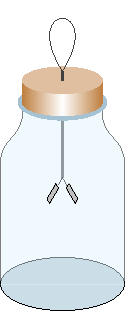
\includegraphics{fig/B/9-15.pdf}
    \caption{}\label{fig_B_9-15}
\end{figure}

照上面说的那样,自己做
一个验电器,要注意,应把瓶盖
擦干净,不能潮湿,以保证它有良好的绝缘性能.利用你自制的验电器,以及塑料尺子、金属小筒、金属网等器材,做一做摩擦起电、感应起电、导体上的电荷分布、静电屏蔽等实验.

\section{自制电池}
把不同的金属放在电解质溶液中,由于化学作用,产生了电动势,就成为一个化学电源.现在把同样大小的四、五个光洁的锌片和钢片交替相叠,并在锌片和钢片之间夹一片吸满盐水的吸水纸,这样就做成了一个简单的电池,锌片和锌片相连是电池的负极,铜片和铜片相连是电池的正极.

用细漆包线在指南针外壳上绕50圈,当漆包线中有电流通过时,磁针发生偏转,这样用指南针就可以检验有无电流.

把漆包线两端的漆刮掉,露出铜丝,分别接在自制电池组的两极上,检验导线中有无电流通过.

\section{研究电灯泡的电阻}
取一只电灯泡,看一看它上面标明的额定功率和额定电压是多少,并利用额定功率和额定电压的数值算出灯丝的电阻.你计算得出的电阻是多少?

再用万用表直接测出这只电灯泡灯丝的电阻,你测得的电阻又是多少?跟计算得出的数值是否一致?想想看,这是什么道理?



